% kapitel2.tex
\chapter{Stand der Forschung}
In diesem Kapitel wird der aktuelle Stand der Forschung des Internets der Dinge erläutert. Es wird besonders auf die Themen Smart Home und Task Automation Services eingegangen, sowie darauf, welche Vorteile sich durch das Kombinieren dieser Ansätze erhoffen lassen.


\section{Internet of Things}
Die Kernideen des modernen Internets der Dinge wurden erstmals Anfang der 90er Jahren des letzten Jahrhunderts aufgeführt. Die Vision, sämtliche intelligenten Geräte in einem vereinten Netzwerk zu integrieren und zu steuern, ist also schon fast drei Jahrzehnte alt. 
Vereinzelt wurden schon damals intelligente Geräte vielerorts in Demonstratoren und Prototypen an das Internet angeschlossen und von Menschen aus der Entfernung gesteuert. Doch erst im Jahre 1999 wurde der Begriff \glqq Internet of Things\grqq{} erstmals von Kevin Ashton, einem der Gründer des Auto-ID Centers am MIT geprägt \cite{iot_history}.\\

Kevin Ashton betrachtete die radio-frequency identification (RFID) Technologie als Grundlage für den Erfolg von IoT. In der Tat fand RFID in den 90er Jahren erstmals massenhafte Verbreitung \cite{rfid_history}. Sie erlaubt es über Radio Wellen Informationen zu übertragen. Heutzutage kommt RFID in den verschiedensten Bereichen zum Einsatz.
Mittlerweile haben sich auch andere Kommunikationstechnologien im IoT Umfeld fest etabliert. Dazu gehören unter anderem IEEE 802.11 (oft umgangssprachlich WLAN genannt), Bluetooth und QR Codes. \\

Seitdem wurden zahlreiche Forschungsprojekte mit staatlicher Unterstützung ins Leben gerufen um das Potential des Internets der Dinge zu evaluieren. Besonders im aktuellen Jahrzehnt wird an Themen, wie Smart Cities und Standardisierung aktiv geforscht.\\

Im Jahre 2007 wurde das European Research Cluster on the Internet of Things (IERC) \cite{ierc} von der europäischen Union ins Leben gerufen. Anfangs wurde damit das Ziel verfolgt die Forschung im Bereich RFID zu unterstützen, doch die unterstützten Forschungsprojekte \cite{ierc:portfolios} gingen schnell weit darüber hinaus. \\

\begin{figure}[t]
	\centering
	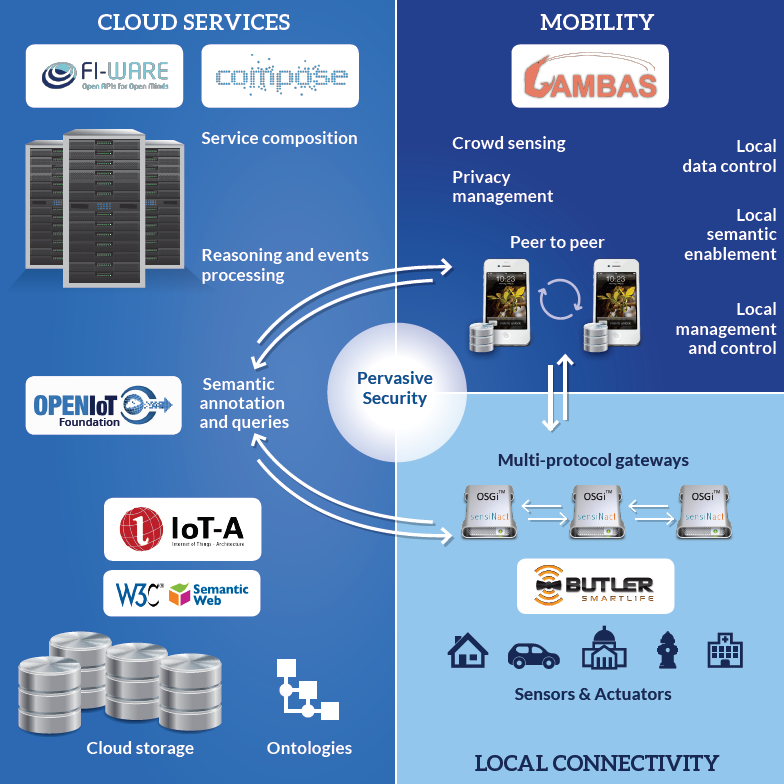
\includegraphics[width=\textwidth]{bilder/ierc}
	\caption{Projektübergreifende Zusammenarbeit der vom IERC unterstützten Forschungsprojekte \cite{ierc:portfolios}. Selbst Teil des Smart Action Projekts \cite{smartAction}}
	\label{fig:ierc}
\end{figure}

Aktuell werden verschiedenste Technologien von Partnern des IERC untersucht. Im Rahmen des Projekts \glqq Internet of Things - Architecture\grqq{} (IoT-A) wurde Anfang des Jahrzehnts ein Architektur-Referenz-Modell (ARM)\cite{iota:d15} entwickelt, das als Grundlage für konkrete IoT Systemarchitekturen dienen sollte. In der Tat kommt es heute in zahlreichen weiterführenden Projekten zum Einsatz. Die gemeinsame Architekturgrundlage sorgt dabei für Interoperabilität und Wiederverwendbarkeit.

In dem Projekt OpenIoT \cite{oiot}, welches im Jahr 2010 ins Leben gerufen wurde, wird die Integration von IoT und Cloud Computing mithilfe von Semantiken untersucht. Unter anderem entstand auf diese Weise eine Open Source Software, die geeignet ist, um Sensoren in eine existierende IoT Lösung zu integrieren.

Einen schematischen Überblick über diese und weitere Forschungsprojekte des European Research Cluster on the Internet of Things liefert Abbildung \ref{fig:ierc}.\\


\begin{figure}[t]
	\centering
	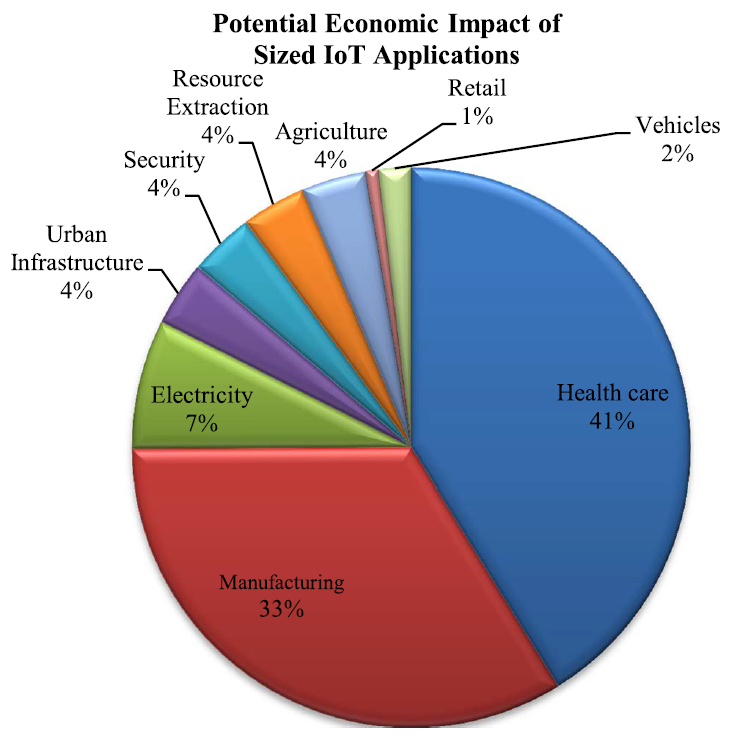
\includegraphics[width=\textwidth]{bilder/iot_market_share}
	\caption{Erwarteter Marktanteil von IoT Anwendungen bis 2025 \cite{IotEnablers}}
	\label{fig:market}
\end{figure}



Nicht nur im Rahmen des IERC wird an IoT geforscht. Die Internationale Fernmeldeunion (engl. International Telecommunication Union, ITU) hat 2013 eine dedizierte Study Group (SG20) ins Leben gerufen, die sich mit den Anwendungsmöglichkeiten von IoT und insbesondere Smart Cities und Communities beschäftigt. Als Teil davon hat die Internet of Things Global Standards Initiative (IoT-GSI) IoT als \textit{globale Infrastruktur einer Informationsgesellschaft} definiert \cite{iot:glob_infr}.  

Auch in wissenschaftlichen Artikeln wird der Begriff IoT aktuell aus verschiedensten Perspektiven betrachtet. Es wird geprüft, inwiefern durch Kombination mit anderen Technologien ein Mehrwert erzielt werden kann. Unter anderem werden Technologien, wie Cloud Computing\cite{FiCloud:CloudIot}, Machine-2-Machine\cite{FiCloud:M3Iot} und Semantic Web\cite{SemWebIoT} kritisch analysiert. An dieser Stelle lässt sich auch diese Masterarbeit in den historischen Kontext einordnen. \\

In der Tat sind die Anwendungsmöglichkeiten des Internets der Dinge sehr vielseitig. Es wird angenommen, dass bis zum Jahre 2025 die globalen ökonomischen Auswirkungen von 2,7 bis 6,2 Trillionen US-Dollar betragen werden \cite{money}. In welchen Bereichen die größten Effekte zu erwarten sind, zeigt Abbildung \ref{fig:market}.


%Wie zu sehen ist, sind die Bereiche Gesundheitspflege und Produktionstechnik am meisten betroffen. 

%Die enorm steigende Anzahl von „intelligenten Gegenständen“ mit eingebetteten Computern, die den Menschen im alltäglichen Leben unterstützen sollen, hat zu der Prägung des Begriffs „Internet der Dinge“ (IoT) geführt. Jedes dieser Dinge hat seine eigene Funktionalität und im Verbund stellen sie eine große Menge an Daten zur Verfügung. Im Rahmen von zahlreichen Forschungsprojekten \cite{ierc:portfolios} werden Möglichkeiten untersucht, IoT mit unterschiedlichen Technologien zu kombinieren. Unter anderem werden Technologien, wie Cloud Computing\cite{FiCloud:CloudIot}, Machine-2-Machine\cite{FiCloud:M3Iot} und Semantic Web\cite{SemWebIoT} kritisch betrachtet. 

%Im Laufe der Zeit haben sich verschiedene Aspekte des IoT herausgebildet, unter anderem das Smart Home.

\subsection{Smart Home}
Ein mit IoT eng verwobenes Thema ist das Smart Home\cite{SmartHomeIoT}, welches die elektronische Steuerung von ausgewählten Geräten mit z.B. einer Rule Engine kombiniert um eine Automatisierung des Geräteverhaltens in einem Zusammenspiel zwischen Sensorik und Aktorik zu erreichen. Smart Home grenzt sich vom übergreifenden IoT-Bereich ab indem es auf Sensoren und Aktoren spezialisiert ist, die im Kontext eines Hauses relevant sind.\\

Bis dato wurden zahlreiche Smart Home Lösungen von verschiedenen Anbietern entwickelt. Man kann prinzipiell zwei Arten von Lösungen unterscheiden. \textit{Proprietäre} Produkte (z.B. \textit{RWE SmartHome} \cite{RWE}) spezialisieren sich auf eine sehr begrenzte Anzahl von Geräten und bemühen sich maximale Unterstützung für diese Geräte zu bieten. Dies sorgt für eine Fragmentierung des Marktes \cite{sh:fragment}. \textit{Open Source} Lösungen hingegen verfolgen das Ziel möglichst offen für verschiedene Geräte und Protokolle zu bleiben.\\ 

Da Open Source Lösungen aktuell noch aktiv in der Entwicklung sind und hauptsächlich als Software existieren, erfordert ihr Einsatz von Nutzern ein gewisses Maß an technischen Vorkenntnissen. In der Regel muss der Nutzer passende Hardware bereitstellen und die Software selbst installieren. Bei Problemen kann Support bestenfalls auf Foren von der Community gefunden werden. 

Diese Gründe führen dazu, dass Open Source Lösungen derzeit noch nicht massenhaft zum Einsatz kommen.



\subsection{Task Automation Services}
\label{subsec:tas}
Die Vereinfachung von Aufgaben ist eines der zentralen Bestreben unseres alltäglichen Lebens. Eine konkrete Ausprägung davon ist die Automatisierung. Sie macht das Leben übersichtlicher und erlaubt uns kostbare Zeit zu sparen. Ob Notifikation auf dem Smartphone, wenn eine Email eingeht oder das Einschalten von Lampen, wenn ein Raum betreten wird, solche Automatisierung ist heutzutage überall zu finden. Lange Zeit musste jede derartige Automatisierung einzeln entworfen, konfiguriert und implementiert werden. Doch die steigende Anzahl von intelligenten Gegenständen und die Allgegenwärtigkeit des Internets überlassen dies der Vergangenheit. Nun hat sich der Ansatz der Task Automation Services\cite{ieee:tas} gebildet.

Ein Task Automation Service (TAS) ist ein Dienst, der es Endnutzern ermöglicht das Verhalten von verschiedenen Services und Geräten in eigenen Szenarien jederzeit selbst zu automatisieren. Solche Szenarien basieren auf Event-Condition-Action (ECA) Regeln\cite{ECA}, welche es ermöglichen, auf Ereignisse unter festgelegten Bedingungen mit entsprechenden Aktionen zu reagieren. Meistens wird dies durch  einen intuitiven visuellen Regel Editor ermöglicht.

%evtl näher eingehen, was typische Charakteristika von TAS sind: Channels, channel paradigms

Aktuell gibt es noch vergleichsweise wenige TAS. Ein Überblick über existierende  Services bietet Abbildung \ref{fig:tasoverview}.

\begin{figure}[h]
	\centering
	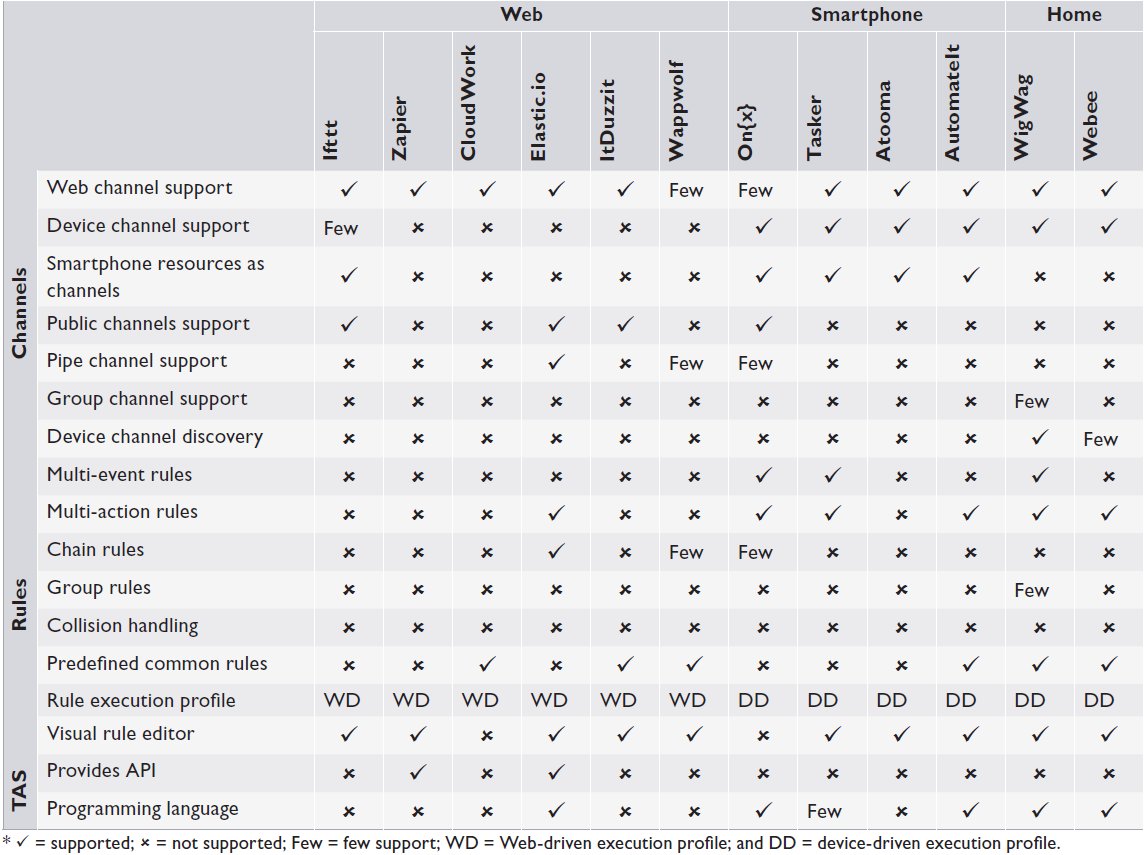
\includegraphics[width=\textwidth]{bilder/TASOverview}
	\caption{Überblick über existierende Task Automation Services \cite{ieee:tas}}
	\label{fig:tasoverview}
\end{figure}

Wie in der Abbildung zu sehen ist, gibt es unterschiedliche Ansätze. Einige TAS sind in der Cloud angesiedelt, was bedeutet, dass sie, sofern Internet verfügbar ist, jederzeit und von überall erreichbar sind. Die aktuell mächtigsten und bekanntesten TAS sind \textit{IFTTT} \cite{IFTTT} und \textit{Zapier}\cite{Zapier}. Sie unterstützen hunderte unterschiedlicher Web Services, bieten aber keine Möglichkeit mit Geräten direkt zu interagieren. Ihr Fokus ist es zu ermöglichen eine Vielzahl von Szenarien auf eine einfache Art und Weise zu erstellen. Auf komplexere Regeln und Szenarien sind ihre Rule Engines nicht ausgelegt. 
Um diese TAS zu nutzen, muss man jedoch bereit sein, sämtliche Zugriffsrechte, die für die zu automatisierenden Dienste (z.B. \textit{Facebook}, \textit{Twitter}, etc.) benötigt werden, dem Cloud Service anzuvertrauen. Dies lässt sich teilweise durch Einsatz von Protokollen wie OAuth und der Übergabe von \textit{eingeschränkten} Rechten mäßigen - dennoch kann der durch einen Angreifer angerichtete Schaden enorm sein.
%TODO beleg

Andere Task Automation Services arbeiten lokal auf Smartphones. Solche TAS konzentrieren sich auf die Automatisierung von den auf dem Gerät laufenden Services. Die Unterstützung von der Automatisierung von Web Services ist nur in dem Umfang gegeben, in dem diese Web Services direkten Kontakt mit dem Smartphone haben.  

Schließlich gibt es TAS, die auf einem dedizierten Gerät im Hause des Endnutzers arbeiten. Solche Task Automation Services konzentrieren sich auf die direkte Steuerung von Geräten mithilfe der entsprechenden Protokolle. Im Grunde sind sie äquivalent zu Smart Home. 

Im Rahmen dieser Arbeit wird Smart Home jedoch getrennt von TAS behandelt, da der Fokus der Automatisierung völlig unterschiedlich ist. Mehr dazu in Sektion \ref{sec:idee}.



\subsubsection{IFTTT}
Ein Beispiel für Task Automation Services in der Cloud ist IFTTT, welches eine große Anzahl verschiedener Services (\textit{Facebook}, \textit{Dropbox}, \textit{Philips Hue}\cite{hue},   etc.) integriert und eine rudimentäre Rule Engine anbietet, die es erlaubt auf eine einfache Art und Weise serviceübergreifende „if this than that“ Anweisungen zu hinterlegen, die der klassischen „EDV“ ähneln. Es wird eine feste Trigger Komponente gewählt, die etwas auslöst, daraufhin wird die Aktion festgelegt, die ausgeführt werden soll. Solche Condition/Command Paare werden in IFTTT \textit{Applets} genannt. 

Bis dato lassen sich komplexere Szenarien mit \textit{IFTTT} nur begrenzt abbilden. Das bedeutet, dass es keine Möglichkeit gibt, beispielsweise, Und- und Oder-Bedingungen zu definieren, die es ermöglichen würden, mehrere Conditions in einem Applet zu verknüpfen. Stattdessen muss komplexes Verhalten in einzelnen Bausteinen auf verschiedene Applets verteilt werden.

Ein weiterer Aspekt von IFTTT ist, dass es für die Anbindung von Services Zugriffsrechte auf sämtliche Accounts des Users bedarf. Aus einer Datenschutz-Perspektive\cite{cloudsec} stellt das ein Risiko für den Endnutzer dar, da diese Zugriffsrechte an einer Stelle gesammelt sind. Im Falle einer Sicherheitslücke bei IFTTT wären alle damit gekoppelten Services in Gefahr. 

\section{Zentrale Idee}
\label{sec:idee}
Wie in Sektion \ref{subsec:tas} zu sehen ist, kann man drei prinzipiell unterschiedliche Arten von Task Automation Services unterscheiden: Cloud Services, Smartphone Applikationen und Smart Home Anwendungen. Sie weisen zwar viele Gemeinsamkeiten auf, doch allein aus den Namen lässt sich ablesen, dass es sich dabei um grundlegend verschiedene Lösungen handelt. 

Die Cloud Services unterstützen nur begrenzt die \glqq direkte\grqq{}  Steuerung von Geräten. Außerdem sind die zum Einsatz kommenden Rule Engines sehr rudimentär. Smart Homes hingegen haben in der Regel mächtige Rule Engines und bieten die Möglichkeit komplexe Szenarien zu definieren. Zusätzlich sind sie in der Lage, Geräte direkt anzusteuern. Im Rahmen dieser Arbeit werden die Smartphone Applikationen nicht näher betrachtet.\\

Die zentrale Idee dieser Arbeit ist es ein Smart Home mit einem Cloud Service TAS zu verschmelzen. Dadurch soll ein Ganzes entstehen, welches mehr ist, als die Summe seiner Teile: Ein (Work-)Flow Automation Service im Kontext Smart Home (FLASH).

\subsection{Ziele}
\label{sec:ziele}
Ziel dieser Arbeit ist es die Welten von Smart Home und webbasierten Task Automation Services zusammen zu bringen. Durch die Integration mit Smart Home soll die direkte Steuerung von Geräten befähigt werden. Außerdem soll die Mächtigkeit der Smart Home Rule Engine genutzt werden, um komplexere Regeln und Szenarien zu ermöglichen. Schließlich sollen die Datenschutzprobleme gelöst werden, indem sämtliche Zugriffsdaten on-premise galagert und dadurch nie einem Risiko ausgesetzt werden.

Es soll ein Demonstrator entwickelt werden, der die Funktionalitäten von Smart Home und TAS kombiniert und in einer on-premise Anwendung anbietet. Hierzu soll das Eclipse SmartHome Framework als Basis verwendet und um Funktionalitäten von webbasierten TAS angereichert werden. Die entstandene Anwendung soll auf einem Raspberry Pi\cite{rasp} laufen.

Die entstandenen Funktionalitäten sollen anhand von einer Reihe von konkreten Services demonstriert werden. Unter anderem sollen ein Wetterdienst, ein Filesharing Service und ein Social Media Service angebunden werden. Die Zusammenarbeit dieser Services untereinander und mit Smart Home Geräten soll anhand von Beispiel-Regeln demonstriert werden. Außerdem soll es möglich sein neue Regeln zum System über eine Benutzeroberfläche hinzufügen zu können.

Zum Schluss soll der entstandene Demonstrator evaluiert werden. Es soll geprüft werden, inwiefern Task Automation Services als on-premise Lösung sinnvoll sind unter Betrachtung von Aspekten wie Reaktionszeiten und Netzwerklast. Hierzu soll ein Vergleich der erstellten Anwendung mit \textit{IFTTT} stattfinden.

\subsection{Konkrete Anforderungen}
\label{sec:anforderungen}
In dieser Sektion werden aus den oben genannten Zielen konkrete Anforderungen an den resultierenden Demonstrator abgeleitet und im Detail festgehalten.

Es wird postuliert, dass der Demonstrator folgende Eigenschaften erfüllt:
\begin{enumerate}

\item Der Demonstrator soll intern wie eine Smart Home Zentrale agieren und in der Lage sein, Geräte innerhalb des Hauses auch ohne Internetverbindung steuern zu können.
\item Bei vorhandener Internetverbindung soll er in der Lage sein ausgewählte  webbasierte Dienste zu automatisieren.
\item Sämtliche (Zugriffs-)Daten sollen lokal auf dem Gerät gelagert werden. 
\item Die Webdienste sollen nahtlos in die Rule Engine integriert werden, sodass komplexe Szenarien ermöglicht werden.
\item Es soll eine grafische Benutzeroberfläche angeboten werden, in der der Nutzer in der Lage ist eigene Szenarien zur Laufzeit zu definieren.
\item Er soll on-premise auf einem Raspberry Pi 3 Model B laufen.

\end{enumerate}

\subsubsection{Anzubindende Services}
\label{subsec:anzubindende_services}
Im Rahmen der Arbeit sollen folgende populäre Internetdienste in den Demonstrator exemplarisch integriert werden:
\begin{enumerate}
\item \textbf{Dropbox}\cite{dropbox} Es soll möglich sein, automatisch Dateien in die Dropbox zu speichern, sowie auf das Ändern von existierenden Dokumenten zu reagieren.
\item \textbf{Twitter}\cite{twitter} Der Demonstrator soll in der Lage sein für den Nutzer Tweets zu schreiben, sowie auf Tweets zu reagieren. Beispielsweise soll es möglich sein, Medien in Tweets automatisch in die Dropbox zu speichern.
\item \textbf{Wetterdienst}\cite{wetterapi} Es sollen Wetterdaten aus dem Internet bezogen und auf konkrete Wetterbedingungen reagiert werden können.
\item \textbf{Email} Der Demonstrator soll in der Lage sein an beliebige Adressen Emails zu versenden.
\end{enumerate}



